\section{Architecture}
\label{section:architecture}

\begin{figure*}[t]
    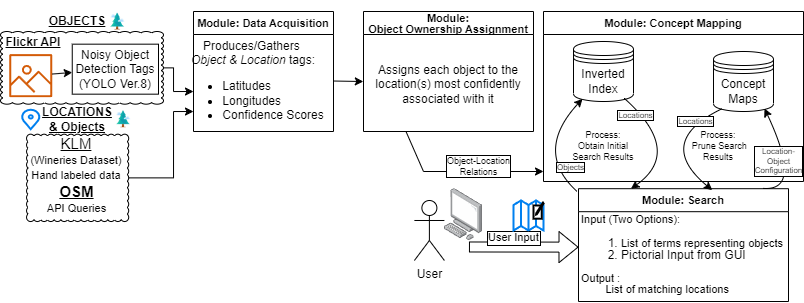
\includegraphics[width=\textwidth]{gestalt_architecture.png}
    \centering
    \caption[width=\textwidth]{The architecture of \emph{GESTALT} consists of the data collection subsystem, the ownership assignment process, the concept mapping process and the search subsystem.}
    \label{fig:architecture}
\end{figure*}

The architecture of \textit{GESTALT} is outlined in Figure \ref{fig:architecture}. The components cover four essential functions: data acquisition, object ownership assignment, concept mapping, and search. 
We describe and motivate each of them below, focusing on their core purposes and leaving the implementation details for sections \ref{section:data} through \ref{section:search}. 

\subsection{Data Acquisition}
%When humans perform last-mile search, they use data from different sources, including overhead imagery, street-view photos, and more.
The Data Acquisition subsystem of \emph{GESTALT} leverages a variety of data sources to ingest objects and locations, including hand-labeled data in KML files, crowd-sourced object and location labels from OSM, and automatically generated object tags we extract from Flickr images geolocated within our region of interest. 
The focus of this component of \emph{GESTALT} is to fuse data in various formats from various sources into a common format so the data can be transformed and searched.
%, aiming to maximize the recall of all possible objects. 
%\emph{GESTALT} currently supports ingestion of hand-labelled objects from KML Files, crowd-sourced object labels from OSM and automatically generated object tags we extract from images geolocated within our region of interest by Flickr.
%All of these data sources are fused into a common format and assigned porbabalistic scores reflecting the likelihood that the object detected is actually present in the real world at the location tagged. 
%The Data Acquisition subsystem ends when all of the data sources have been stored as JSON files, ready for ingestion by the Ownership Assignment subsystem. 

\subsection{Ownership Assignment}
The Ownership Assignment subsystem of \emph{GESTALT} maps the \textit{objects} to the \textit{locations} they most likely belong to using a fuzzy clustering that allows objects to be assigned to multiple locations. 
We use DBSCAN~\cite{DBSCAN} to cluster the objects on the first pass and prune out noisy objects that are unlikely to be associated with any particular location. % by assigning them to a \textit{Null Cluster}. 
The resulting cluster centroids are then mapped to locations based on proximity using a nearest-neighbor search on a KD-Tree, and objects are added to nearby clusters using an adjustable 'fuzziness' parameter.
This assignment protocol is designed to account for uncertainty in tag coordinates of locations and objects and allow for the possibility that objects can be visible from multiple locations in the real world.

%The system accepts a JSON file of \textit{locations} and a series of JSON files of geolocated \textit{objects} both generated by the Data Acquisition subsystem. 
%instantiated into a KD-Tree with the location centroids and a nearest-neighbor search determines what location is closest to that cluster of objects, and assigns it as the parent \textit{location} for that \textit{object cluster}.
%The Ownership Assignment subsystem returns a dataframe of objects, their predicted parent locations and their respective coordinates. 

\subsection{Concept Mapping}
The Concept Mapping subsystem of \emph{GESTALT} creates the data structures (inverted index, location-object concept map, object-object concept map) that enable successive pruning and spatial searching of objects and locations. 
The inverted index maps each object class to the set of locations that contain objects of that type, enabling membership queries to prune the search space for downstream spatial searching. 
The location-object concept map treats the coordinates of the \textit{location} as the division point on both the north-south and west-east axes, and maps the objects for each location to the quadrant that specifies the cardinal direction they lie in with respect to the location.% (NW, NE, SW and SE). 
The object-object concept map (for each location) relates each object to every other object. These take the form of sparse M x M matrices, where M is the number of objects assigned to the location, and an object at position [i,j] is the i$^{th}$ object from the north and the j$^{th}$ object from the west. 

%makes no assumptions about the position of the objects relative to the location, and rather 
%The object-object concept map is sparse M x M matrix, where M is the number of objects assigned to the location, and an object at position [i,j] is the i$^th$ object from the north and the j$^th$ object from the west. 
%The concept mapping subsystem returns these three data structures - the object inverted index, the location-object indexes and the object-object matrices. 
%Each list contains the objects belonging to that location which reside in that quadrant, relative to the location centroid. 
%If the object doesn't exist at a location, there is no point in searching for its relative location.
%The Concept Mapping subsystem accepts as input the objects and their predicted parent locations. 
%Using the input dataframe, the subsystem creates two distinct data structures, intended to support different types of spatial queries. 

\subsection{Search}

The Search subsystem of \emph{GESTALT} enables the user to identify locations of interest based on partial knowledge about the collection and geospatial arrangement of objects at that location. 
The search process is designed for the way humans naturally conceptualize and describe locations and directions- by drawing a sketch map.
Queries can be issued either using keywords and cardinal relations (like Northwest, Southeast, etc.) or using a pictorial specification, where objects can be added and visually arranged in a configuration that is then matched against the concept maps.
The Search subsystem supports fuzzy searching to return inexact matches when query terms are too narrowly defined and ranking to reflect the uncertainty in any given object's identification, tagging, and assignment to a location.

%including the pictorial specification of queries, leveraging the human tendency to draw scratch-maps to describe locations and directions.
%It accepts as input a user query - either through a keyword search or a pictorial query specification and the three data structures created by the concept mapping subsystem. 
%It is capable of exact and fuzzy searching. 
%The search subsystem balances precision in reducing the number of candidate locations with maximizing the recall of possible candidate locations. 
%The recall is prioritized based on the probability that they are the user's intended location. 



\subsection{Summary of Architecture}
The Architecture of \textit{GESTALT} is designed to be lightweight and modular. The core requirement is to automate the last-mile search problem and allow users to search for locations of interest based on partial information. 
Achieving this outcome necessitates collecting and processing objects and locations autonomously, at scale.
Given a large quantity of noisy object tags, \emph{GESTALT} performs fuzzy object assignment, allowing for objects to be assigned to multiple nearby locations, and thereby improving the recall of the system.
The subsequent concept mapping and spatial search processes maintain the system's precision using the relative directional relationships between query objects to extract implicit information about the location the user seeks. 